\documentclass[../main.tex]{subfiles}

%TODO

\begin{document}
	
\chapter{Розробка і тестування системи}
	
\section{Розробка  системи}
	
\subsection{Обґрунтування вибору засобів реалізації}

\textbf{Операційна система.}
Існує декілька найпоширеніших операційних систем для смартфонів, такі як Android, IOS та ін. Для розробки додатку за темою дипломної роботи було обрано операційну систему Android, тому що: 
\begin{itemize}[label={--}]
	\item вона має відкритий вихідний код;
	\item частка пристроїв на Android значно більша, ніж на інших операційних системах (див. рис. \ref{chart:market_share});
	\item абсолютно безкоштовна для розробки.
\end{itemize}

\begin{figure}[H]
	\centering
	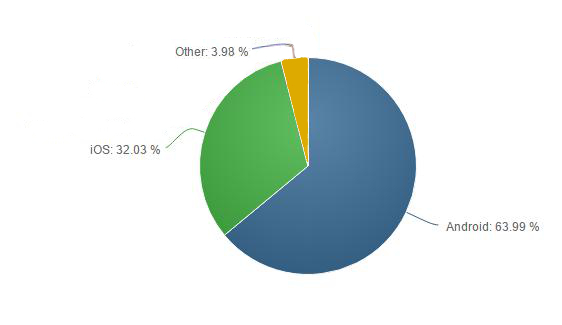
\includegraphics[width=1\textwidth]{market_share_2016}
	\caption{Частка пристроїв на різних ОС станом на 2016 рік}
	\label{chart:market_share}
\end{figure}

Також, було обрано мінімальну версію API для розробки додатку. Як видно з рис. \ref{chart:android_versions}, пристроїв під керуванням Android нижче версії API 19 досить мало, тому можна було б їх проігнорувати, та встановити її як мінімальну. Однак, для розроблюваного додатку для цього немає гострої необхідності, тому було обрано API версії 16 як мінімальну.\\

\begin{figure}[H]
	\centering
	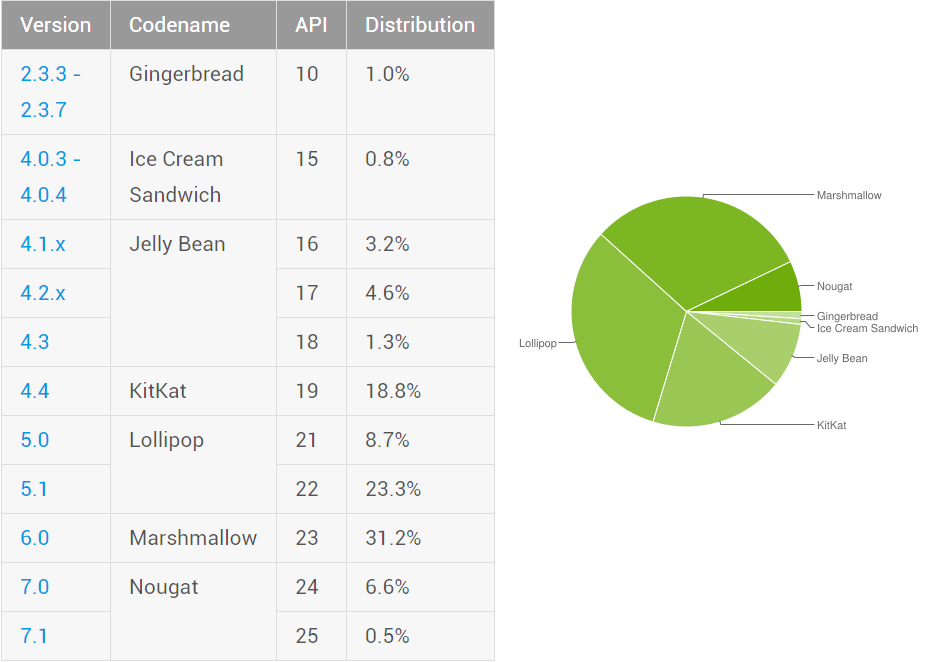
\includegraphics[width=1\textwidth]{android_versions}
	\caption{Відносна кількість пристроїв, що працюють під управлінням різних версій Android}
	\label{chart:android_versions}
\end{figure}

\textbf{Мова програмування.} 
В якості мови програмування для реалізації Android-щоденника було обрано мову Java. Ця мова повністю об'єктно-орієнтована. Всі сутності в Java є об'єктами, за виключенням основних (примітивних) типів: boolean, int, long, double і т.д. 

Розробниками Java був проведений фундаментальний аналіз програм на мові C++. В результаті цього аналізу вони вилучили можливість явного виділення і звільнення пам'яті. Наприклад, пам'ять в Java звільняється автоматично за допомогою механізму збору сміття (garbage collection), тому розробник застрахований від помилок, що виникають під час неправильного використання пам'яті. Однією з особливістей Java є відсутність множинного наслідування. Замість цього існує можливість імплементувати декілька інтерфейсів.

У тому числі, засоби для розробки під операційну систему Android написані на Java та більшість документації для Android містить приклади коду на цій мові.

\textbf{Середовище розробки.}
В якості середовища розробки було обрано Android Studio IDE, так як вона офіційна та постійно оновлюється. Серед функцій, що є в Android Studio, можна виділити такі:

\begin{enumerate}
	\item Розширений редактор макетів, що дозволяє працювати з компонентами користувацього інтерфейсу за допомогою перетягування їх на поле, що представляє екран пристрою. Також присутня функція попереднього перегляду макету при різних конфігураціях екрану.
	\item Збирання проектів основане на Gradle.
	\item Потужні інструменти для рефакторингу.
	\item Статичний аналізатор коду (Lint), що дозволяє знаходити проблеми продуктивності, несумісності версій та інших проблем.
	\item Різні види збірок та генерація декількох .apk файлів.
	\item Вбудований ProGuard (утиліта, призначена для оптимізації та обфускації Java коду), та утиліта для підпису додатків.
	\item Шаблони основних макетів та компонентів Android.
	\item Вбудована підтримка Google Cloud Platform, котра включає в себе інтеграцію з сервісами Google Cloud Messaging та App Engine.
	\item Підтримка останніх весрій Android SDK, в тому числі і Preview версій.
	\item З версії 2.1 підтримує оновлений компілятор Jack, також було покращено підтримку Java 8.
	\item Підтримка розробки додатків для Android Wear та Android TV.
\end{enumerate}

%TODO: add screenshots

\textbf{База даних.}
Для роботи з базою даних було вирішено використовувати сервіс Firebase. Він являє собою постачальника хмарних сервісів і додатків. Головний офіс знаходиться в Сан-Франциско, Каліфорнія. У 2011 році Andrew Lee і James Tamplin заснували Firebase і в квітні 2012 запустили хмарний сервіс. Основний напрямок Firebase -- хмарна noSQL база даних для real-time додатків (що працюють в режимі реального часу), яка надає API, що дозволяє розробникам зберігати та синхронізувати дані між декількома клієнтами. У жовтні 2014 року компанія була придбана Google, та у травні 2016 на конференції Google I/O було представлено значну кількість нових функцій.

Firebase надає real-time базу даних як сервіс, що в свою чергу має API для розробників, котра дозволяє синхронізувати дані додатку між клієнтами та зберігати їх у хмарі Firebase (див. рис. \ref{figure:firebase_workflow}). Компанія надає клієнтські бібліотеки, які дозволяють інтеграцію з Android, IOS, JavaScript, Java, Objective-C, Swift та Node.js додатками. Робота безпосередньо з базою даних реалізована через REST сервіси для деяких JavaScript фрейморків, таких як AngularJS, React, Ember.js і Backbone.js. REST API використовує протокол Server-Sent Events (SSE). Розробники, що використовують цю БД можуть захистити свої дані за допомогою встановлення правил безпеки на стороні серверу \cite{firebase_secure}.

\begin{figure}[H]
	\centering
	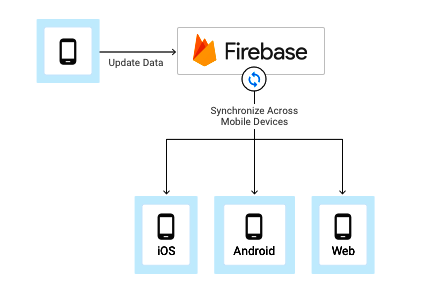
\includegraphics[width=0.8\textwidth]{firebase_workflow}
	\caption{Принцип роботи real-time бази даних Firebase}
	\label{figure:firebase_workflow}
\end{figure}

Основні можливості бази даних Firebase:
\begin{enumerate}
	\item \textit{Миттєва синхронізація.} Замість типових запитів HTTP, real-time база даних Firebase використовує синхронізацію даних -- кожен раз, коли дані змінюються, будь-який підключений пристрій отримує ці оновлення миттєво.
	\item \textit{Автономність.} Firebase додатки залишаються працездатним навіть в автономному режимі, так як Firebase SDK зберігає дані на диск. Після того, як підключення буде відновлено, пристрій клієнту отримає всі зміни, що було пропущено, та синхронізується з поточним станом сервера.
	\item \textit{Зручний доступ з пристроїв клієнтів.} Доступ до бази даних Firebase можна отримати безпосередньо з мобільного пристрою або веб-браузеру, немає необхідності для серверу. Безпека та перевірка даних доступні через правила безпеки для бази даних Firebase -- основані на виразах правила, котрі виконуються, коли дані зчитуються або записуються.
\end{enumerate}

База даних Firebase являє собою noSQL базу і має різні оптимізації та функціональні можливості в порівнянні з реляційною базою. API бази Firebase побудована так, щоб дозволити тільки операції, котрі можуть бути виконані швидко. Це дозволяє будувати чудові real-time рішення, що можуть служити мільйонам користувачів без шкоди для гнучкості. Через це, важливо думати про те, як користувачі повинні отримувати доступ до даних, а потім структурувати їх відповідним чином.

Для збереження файлів Firebase надає зручний сервіс Cloud Storage -- потужний, простий та рентабельний сервіс для збереження об'єктів. Firebase SDK для хмарного збереження даних додає безпеки до процесу вивантаження та завантаження файлів для Firebase додатків, незалежно від якості мережі. Також, є можливість використовувати цю SDK для зберігання зображень, аудіо, відео або іншого контенту, що створюють користувачі. На сервері, можна використовувати Google Cloud Storage, щоб отримати доступ до тих же файлів.

%TODO: add info about Firebase Auth

Також, Firebase має безліч інших інструментів для розробників (див. рис. \ref{figure:firebase_tools}), якими користуються такі компанії, як The New York Times, Shazam, duolingo, Alibaba.com та інші \cite{firebase}.

%TODO: add info about Goole Location, Maps, Places

\begin{figure}[H]
	\centering
	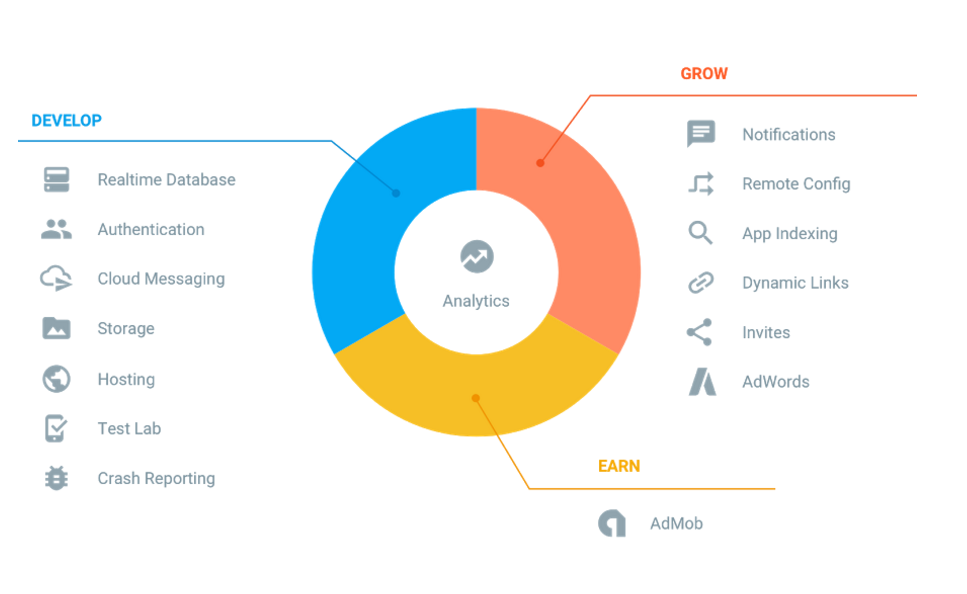
\includegraphics[width=1\textwidth]{firebase_tools}
	\caption{Набір інструментів Firebase}
	\label{figure:firebase_tools}
\end{figure}

\subsection{Опис структурної (функціональної) схеми}

\subsection{Опис логічної схеми}

\subsection{Розробка бази даних}

\subsection{Розробка інтерфейсу користувача}

\subsection{Опис розробки програмних компонентів}

\section{Тестування інформаційної системи}

\section{Висновки}

% TODO: Висновки до розділу (не більш 1-2 сторінки). Розмір одного висновку приблизно – один абзац (5-7 рядків).
	
\end{document}